\section{Adaptive Learning Algorithms}

% --------------------------------------------------------------------------------------------------------------
\begin{frame}
\frametitle{The setting}



\end{frame}
% --------------------------------------------------------------------------------------------------------------

% --------------------------------------------------------------------------------------------------------------
\begin{frame}[allowframebreaks]
\frametitle{Concept drift}
\begin{de}{Concept drift}
Formally, concept drift between time point $t_0$ and time point $t_1$ can be defined as:
$$\exists X:p_{t_0}(X,y) \neq p_{t_1}(X,y)$$

where $p_{t_0}$ denotes the joint distribution at time $t_0$ between the set of input variables X and the target variable y.
\end{de}

Changes in data:

\begin{itemize}
\item prior probablities of classes $p(y)$ may change.
\item class conditional probabilites $p(X|y)$ may change
\item as a result the posterior probablities of classes $p(y|X)$ may change (afftects the prediciton).
\end{itemize}

\framebreak
$$\exists X:p_{t_0}(X,y) \neq p_{t_1}(X,y)$$
\begin{de}{Real concept drift}
refers to changes in $p(y|X)$. Such changes can happen either with
or without change in $p(X)$. It's also called \textit{concept shift} or \textit{conditional change}.
\end{de}

\begin{de}{Real concept drift}
refers to changes in $p(y|X)$. Such changes can happen either with
or without change in $p(X)$. It's also called \textit{concept shift} or \textit{conditional change}.
\end{de}
\end{frame}
% --------------------------------------------------------------------------------------------------------------


% --------------------------------------------------------------------------------------------------------------
\begin{frame}
\frametitle{Example: real vs. virtual drift}
\begin{figure}
	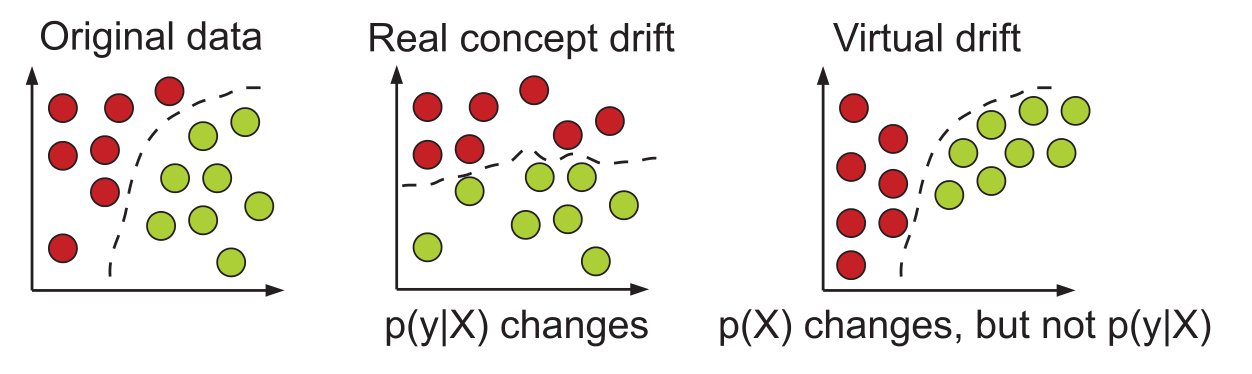
\includegraphics[width=\textwidth]{types}
\end{figure}
\textit{Circles} represent instances.\\
Different \textit{colors} represent different classes.

\end{frame}
% --------------------------------------------------------------------------------------------------------------

% --------------------------------------------------------------------------------------------------------------
\begin{frame}[allowframebreaks]
\frametitle{A practical example: \# of people in a library}
\begin{figure}
	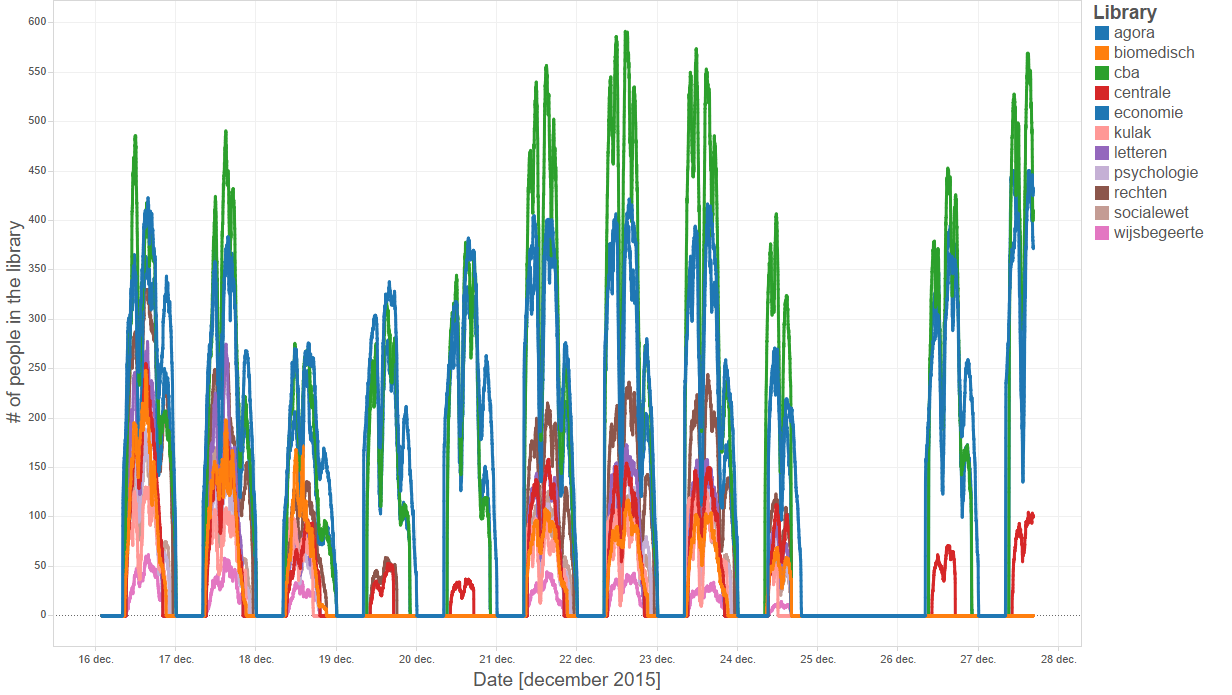
\includegraphics[width=\textwidth]{general_all}
	\caption	{\# of people in the KU Leuven libraries}
\end{figure}

\end{frame}

\begin{frame}

\begin{figure}
	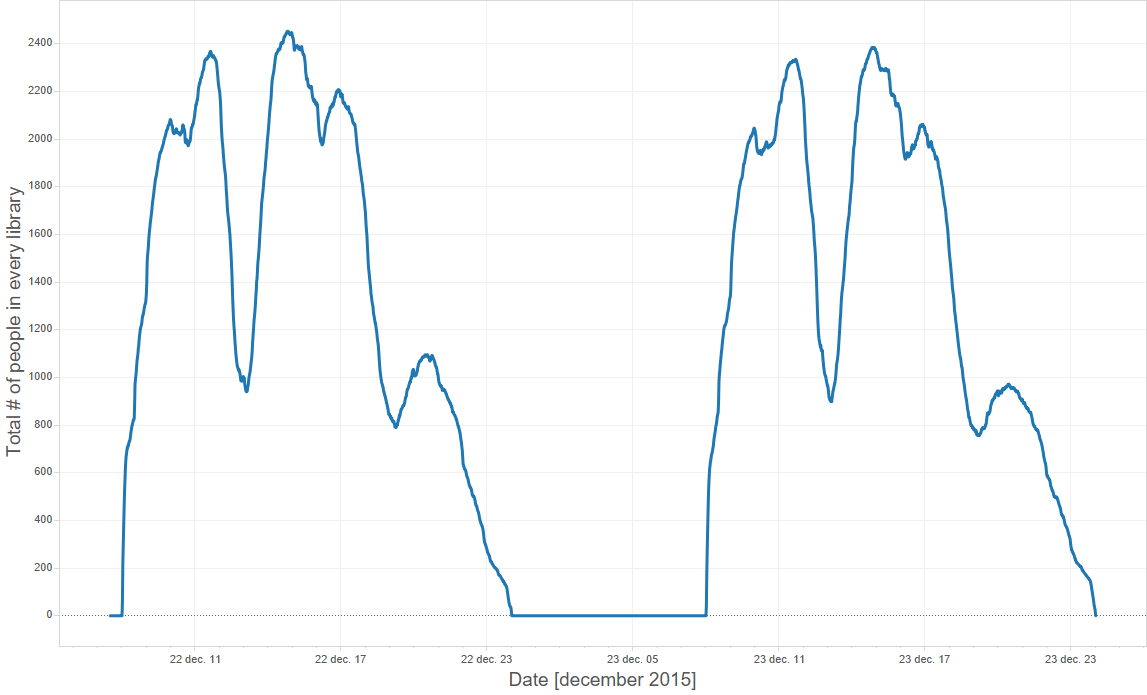
\includegraphics[width=0.75\textwidth]{total}
	\caption	{Sum of people in all KU Leuven libraries}
\end{figure}
\textbf{Task:} predict the total amount of people in all libraries\\
If same amount of people go to different libraries: \only<2>{$\rightarrow$ virtual drift}
\end{frame}
% --------------------------------------------------------------------------------------------------------------
\begin{frame}

\begin{figure}
	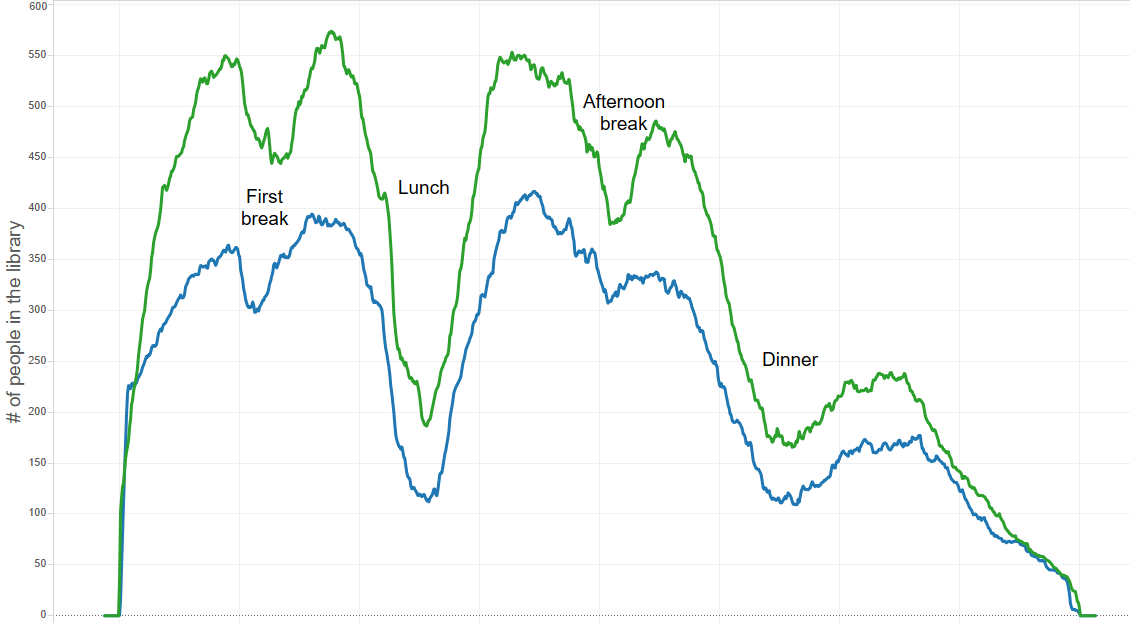
\includegraphics[width=0.75\textwidth]{comparison}
	\caption	{Sum of people in all KU Leuven libraries}
\end{figure}
\textbf{Task:} predict percentage of people in a specific library on a monday\\
If some people go to different libraries: \only<2>{$\rightarrow$ real drift}
\end{frame}